All agents in our network have a fixed \textit{memory length}, i.e. they can remember a maximum
 amount of news.
In this section, its influence in network topology will be studied: clustering and
 diameter are standard measures in network science's literarure and widely used to describe 
 network properties.\\
  Each of them will be plotted 
 against memory length to search possible correlations.
\subsection{Clustering} \label{clustering}
A large number of networks show a tendency for link formation between neighboring vertices, 
i.e., the network topology deviates from uncorrelated random networks: this tendency is called 
\textit{clustering} \cite{clusterarticle}. \\
For unweighted graphs, the clustering of a node $u$ is the fraction of possible triangles over 
all possible triplets  through that node that exist \cite{clustersite},

\begin{equation}
\label{eq:clustering}
c_u = \frac{2 T(u)}{deg(u)(deg(u)-1)}
\end{equation}
where $T(u)$ is the number of triangles through node $u$ and $deg(u)$ is the degree of $u$.
Hence, the \textit{average clustering coefficient}  is:
\begin{equation}
\label{eq:average_clustering}
ACC = \frac{1}{n}\sum_{v \in G} c_v
\end{equation}
We ask wether memory, previously considered in section \ref{introduction}, could affect the 
average clustering coefficient.
To answer the question, the following experiment was designed:
for every memory size, five simulations were run over a thousand iterations; $ACC$'s mean and 
standard deviation were computed afterwards.\\
Finally, via weighted interpolation, a plot of $ACC$'s mean over memory size will show possible
 correlations. \hl{Results and discussion are reported together with diameter}.
\begin{figure}[h]
  \centering
  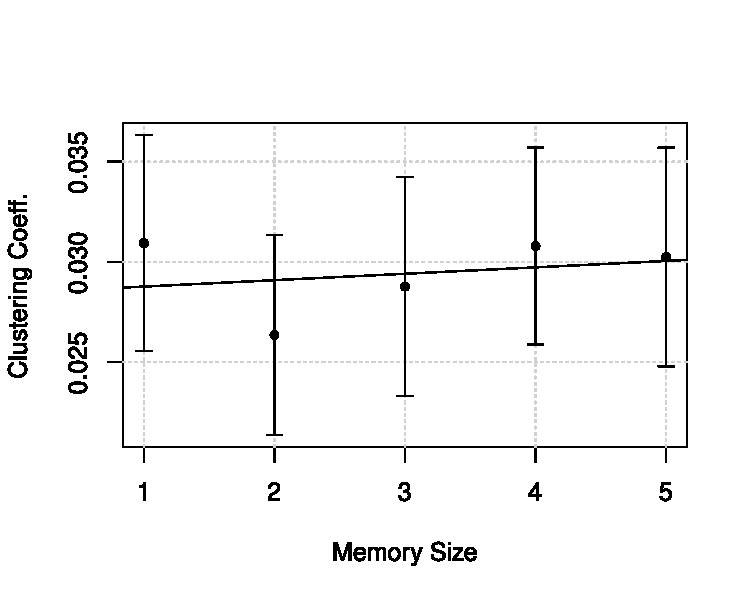
\includegraphics[trim={0cm 0cm 0cm 1cm},clip,width=.8\columnwidth]{img/clustering.pdf}
  \caption{$ACC$'s mean-memory size linear weighted fit: five simulations per point.}
  \label{fig:clustering}
\end{figure}
